\documentclass[conference, letterpaper]{IEEEtran}
\IEEEoverridecommandlockouts
% The preceding line is only needed to identify funding in the first footnote. If that is unneeded, please comment it out.
\usepackage{cite}
\usepackage{geometry}
\usepackage{amsmath,amssymb,amsfonts}
\usepackage{algorithmic}
\usepackage{graphicx}
\usepackage{textcomp}
\usepackage{xcolor}
\usepackage{pgfplots}
\usepackage{tikz}
\usepackage{comment}
\usepackage{multirow}
\geometry{left=0.68in,right=0.68in,top=0.764in,bottom=1.049in}
\pgfplotsset{compat=1.18} 

\def\BibTeX{{\rm B\kern-.05em{\sc i\kern-.025em b}\kern-.08em
    T\kern-.1667em\lower.7ex\hbox{E}\kern-.125emX}}
\begin{document}

\title{Design of a Communication Network for Distributed Renewable Energy Generation Systems\\

}

\author{\IEEEauthorblockN{Fatih DÖNMEZ}
\IEEEauthorblockA{\textit{Kutahya Dumlupinar University} \\
\textit{Faculty of Engineering}\\
\textit{Dept. of Electrical and Electronics Engineering}\\
\textit{Photonics Tech. App. and Res. Center
}\\
Kütahya, Turkey \\
fatih.donmez0@ogr.dpu.edu.tr}
\and
\IEEEauthorblockN{Ahmet ALTUNCU}
\IEEEauthorblockA{\textit{Kutahya Dumlupinar University} \\
\textit{Faculty of Engineering}\\
\textit{Dept. of Electrical and Electronics Engineering}\\
\textit{Photonics Tech. App. and Res. Center
}\\
Kütahya, Turkey \\
altuncu@dpu.edu.tr}

}

\maketitle

\begin{abstract}
Renewable energy systems, which are intermittent energy production systems, cannot always operate at high efficiency due to their nature. Since specific amounts of energy must be spent for energy production, it is essential to estimate the time intervals when the efficiency of the energy source is high. In order to actively monitor the system health, the communication traffic must be transferred to a monitoring room where the technical teams can easily observe the operating data of the equipment in the energy-generating plants. It has been assumed that the energy needs of vocational schools affiliated with the university are met by solar energy systems previously installed by the university administration in their fields. Thanks to the simulation programs, a communication network that does not violate the standards published by the International Electrotechnical Commission for solar energy systems has been designed. Contrary to the methods most preferred in wide area networks like Telecommunication Company's tariff, we preferred wireless communication technologies. By choosing comprehensive area network technology WiMAX and local area network technology WiFi, we passed the required performance criteria under the name of related communication standards.
\end{abstract}

\begin{IEEEkeywords}
Communication networks, wireless sensor networks, Wifi, WiMAX, renewable energy systems, solar energy systems, communication network modelling
\end{IEEEkeywords}

\section{Introduction}
As a result of increasing energy demand and limited fossil fuel resources, studies on renewable energy sources have begun to increase due to increasing carbon dioxide emissions from fossil fuels. %The most effective method of raising awareness of renewable energy systems is training programs for people to get to know renewable energy sources. In this context, schools are the perfect showcase for the benefits of renewable energy. The school's renewable energy system provides students with an on-site learning experience while contributing to the school's energy needs. Students learn about real-world energy issues, including the need to reduce our use of fossil fuels and lower school energy costs. Since solar energy systems' installation, maintenance, repairment, and educational issues are more suitable for students in schools \cite{b1},solar energy systems are mostly preferred as renewable energy by educational institutions.
Sun is one of the cleanest renewable energy resources in the world. Solar panels are being developed to increase their production efficiency by engineers and the scientists. 

There are also negative consequences that come up with the factors that encourage solar energy systems. Approximately 14\% of operating solar energy systems encounter large-scale failures \cite{b2}. Since these faults are significant, they directly affect energy production activities. System failures and factors such as solar radiation value, temperature, environmental pollution, and weather conditions in the regions where the solar energy system is installed directly affect the solar energy performance. A recent study points out that makes it possible to examine the performance status of solar energy systems \cite{b3}.

In \cite{b4} the characteristics of the communication infrastructures used in wind power plants have been investigated. While wired communication technology includes LAN, fiber optic, telecom line, and private data communication, they mentioned that Zigbee, WiFi, WiMAX, satellite, and digital microwave structures are used in wireless technology. Another study shows that it is possible to manage large-scale solar farms with a new Power Line Communication (PLC) communication technique \cite{b5}. In \cite{b6}, the authors designed a communication network based on three different communication technology on small-scale wind and solar systems.

In this paper, the main objective aims to study the communication network architecture for monitoring the behavior of distributed energy generation, including eleven small-scale photovoltaic systems, using different kinds of sensors and communication techniques. 

The photovoltaic system includes voltage, current, wind speed, humidity, irradiation, and temperature informations. We suppose that eleven Photovoltaic (Photovoltaic) systems are belonged to Kütahya Dumlupınar University and facilitated by technical staff, and each Photovoltaic system feeds its vocational school. The previous works generally focused on cabled communications for wide-scale communication in energy systems. For maintenance and error detection, wireless networks are easier than cabled network. Using WiMAX and WiFi technologies, a simulation model is designed using Riverbed Modeler. We evaluated the performance of proposed models given FTP upload response time and a total end-to-end delay in WiFi and WiMAX communication basis. 


The proposed network architecture for Photovoltaic farms is presented in Section 2. The Photovoltaic communication network with data modeling, requirements, and simulation setup is given in Section 3, while the analysis and discussion of simulation results are in Section 4. The concluding remarks and related future work are in Section 5.

\newpage
\newgeometry{left=0.68in,right=0.68in,top=0.75in,bottom=1.049in}
\section{Network Architecture}


The proposed network architecture for Photovoltaic farms is shown in Fig.~\ref{fig:figure1}. It is composed of three layers, namely: Local Photovoltaic System Layer (LPSL), Regional Base Station Layer (RBSL), and Central Control Center Layer (CCCL). Each of the layers is based on a specific function. LPSL is the data generation layer that consists of several modules connected to form a module string. The output voltage of these systems may be affected if a fault in any single module may degrade the system output. Also, other factors may degrade the system performance, such as shading and dust. Different sensor nodes are installed to monitor the system continuously, which enables the detection of any fault and enables rapid response to control the system operation \cite{b6}. Data and states of the Photovoltaic system are designed with modules measuring sensors are shown in Table \ref{tab:table1}. All sensors and data are collected via WiFi and routed via a WiMAX link to the control center with two hops.
\begin{figure}[htbp]
\centerline{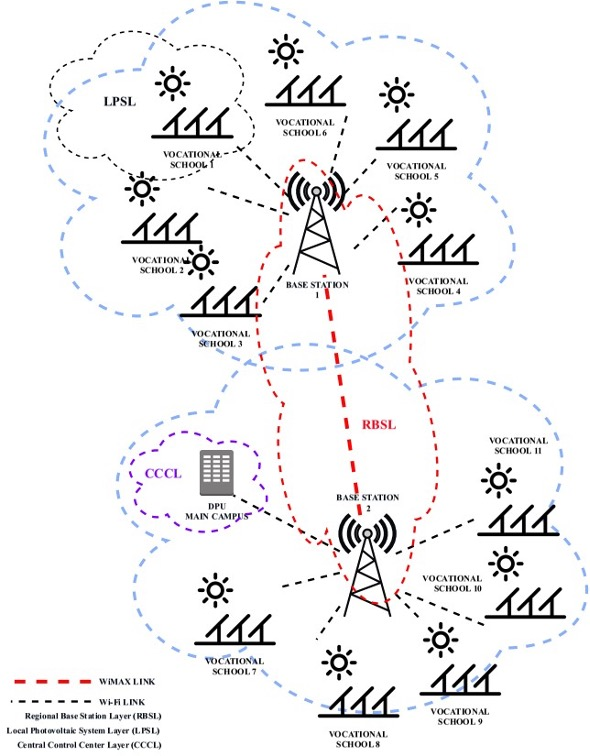
\includegraphics[width=\columnwidth]{figure1.jpg}}
\caption{The proposed communication network topology of Dumlupinar University main and sub-campuses and their base stations.}
\label{fig:figure1}
\end{figure}

Suppose LPSL has 44 WiFi-based sensors for just a vocational school. The total sensor number is 484 for the entire vocational school network at Kütahya Dumlupinar University. Those sensors communicate directly to their Access Points and indirectly to the CCCL.


RBSL is the bridge between the LPSL and CCCL. The data from LPSL are collected and transmitted to CCCL in this layer. Each LPSL has its subscriber unit configured and connected to its base station in the WiMAX structure. In this scenario, we analyzed the proper locations for base stations. All vocational schools and the central campus are communicating with their base station at Line of Sight (LOS).
\begin{comment}
\begin{figure}[htbp]
\centerline{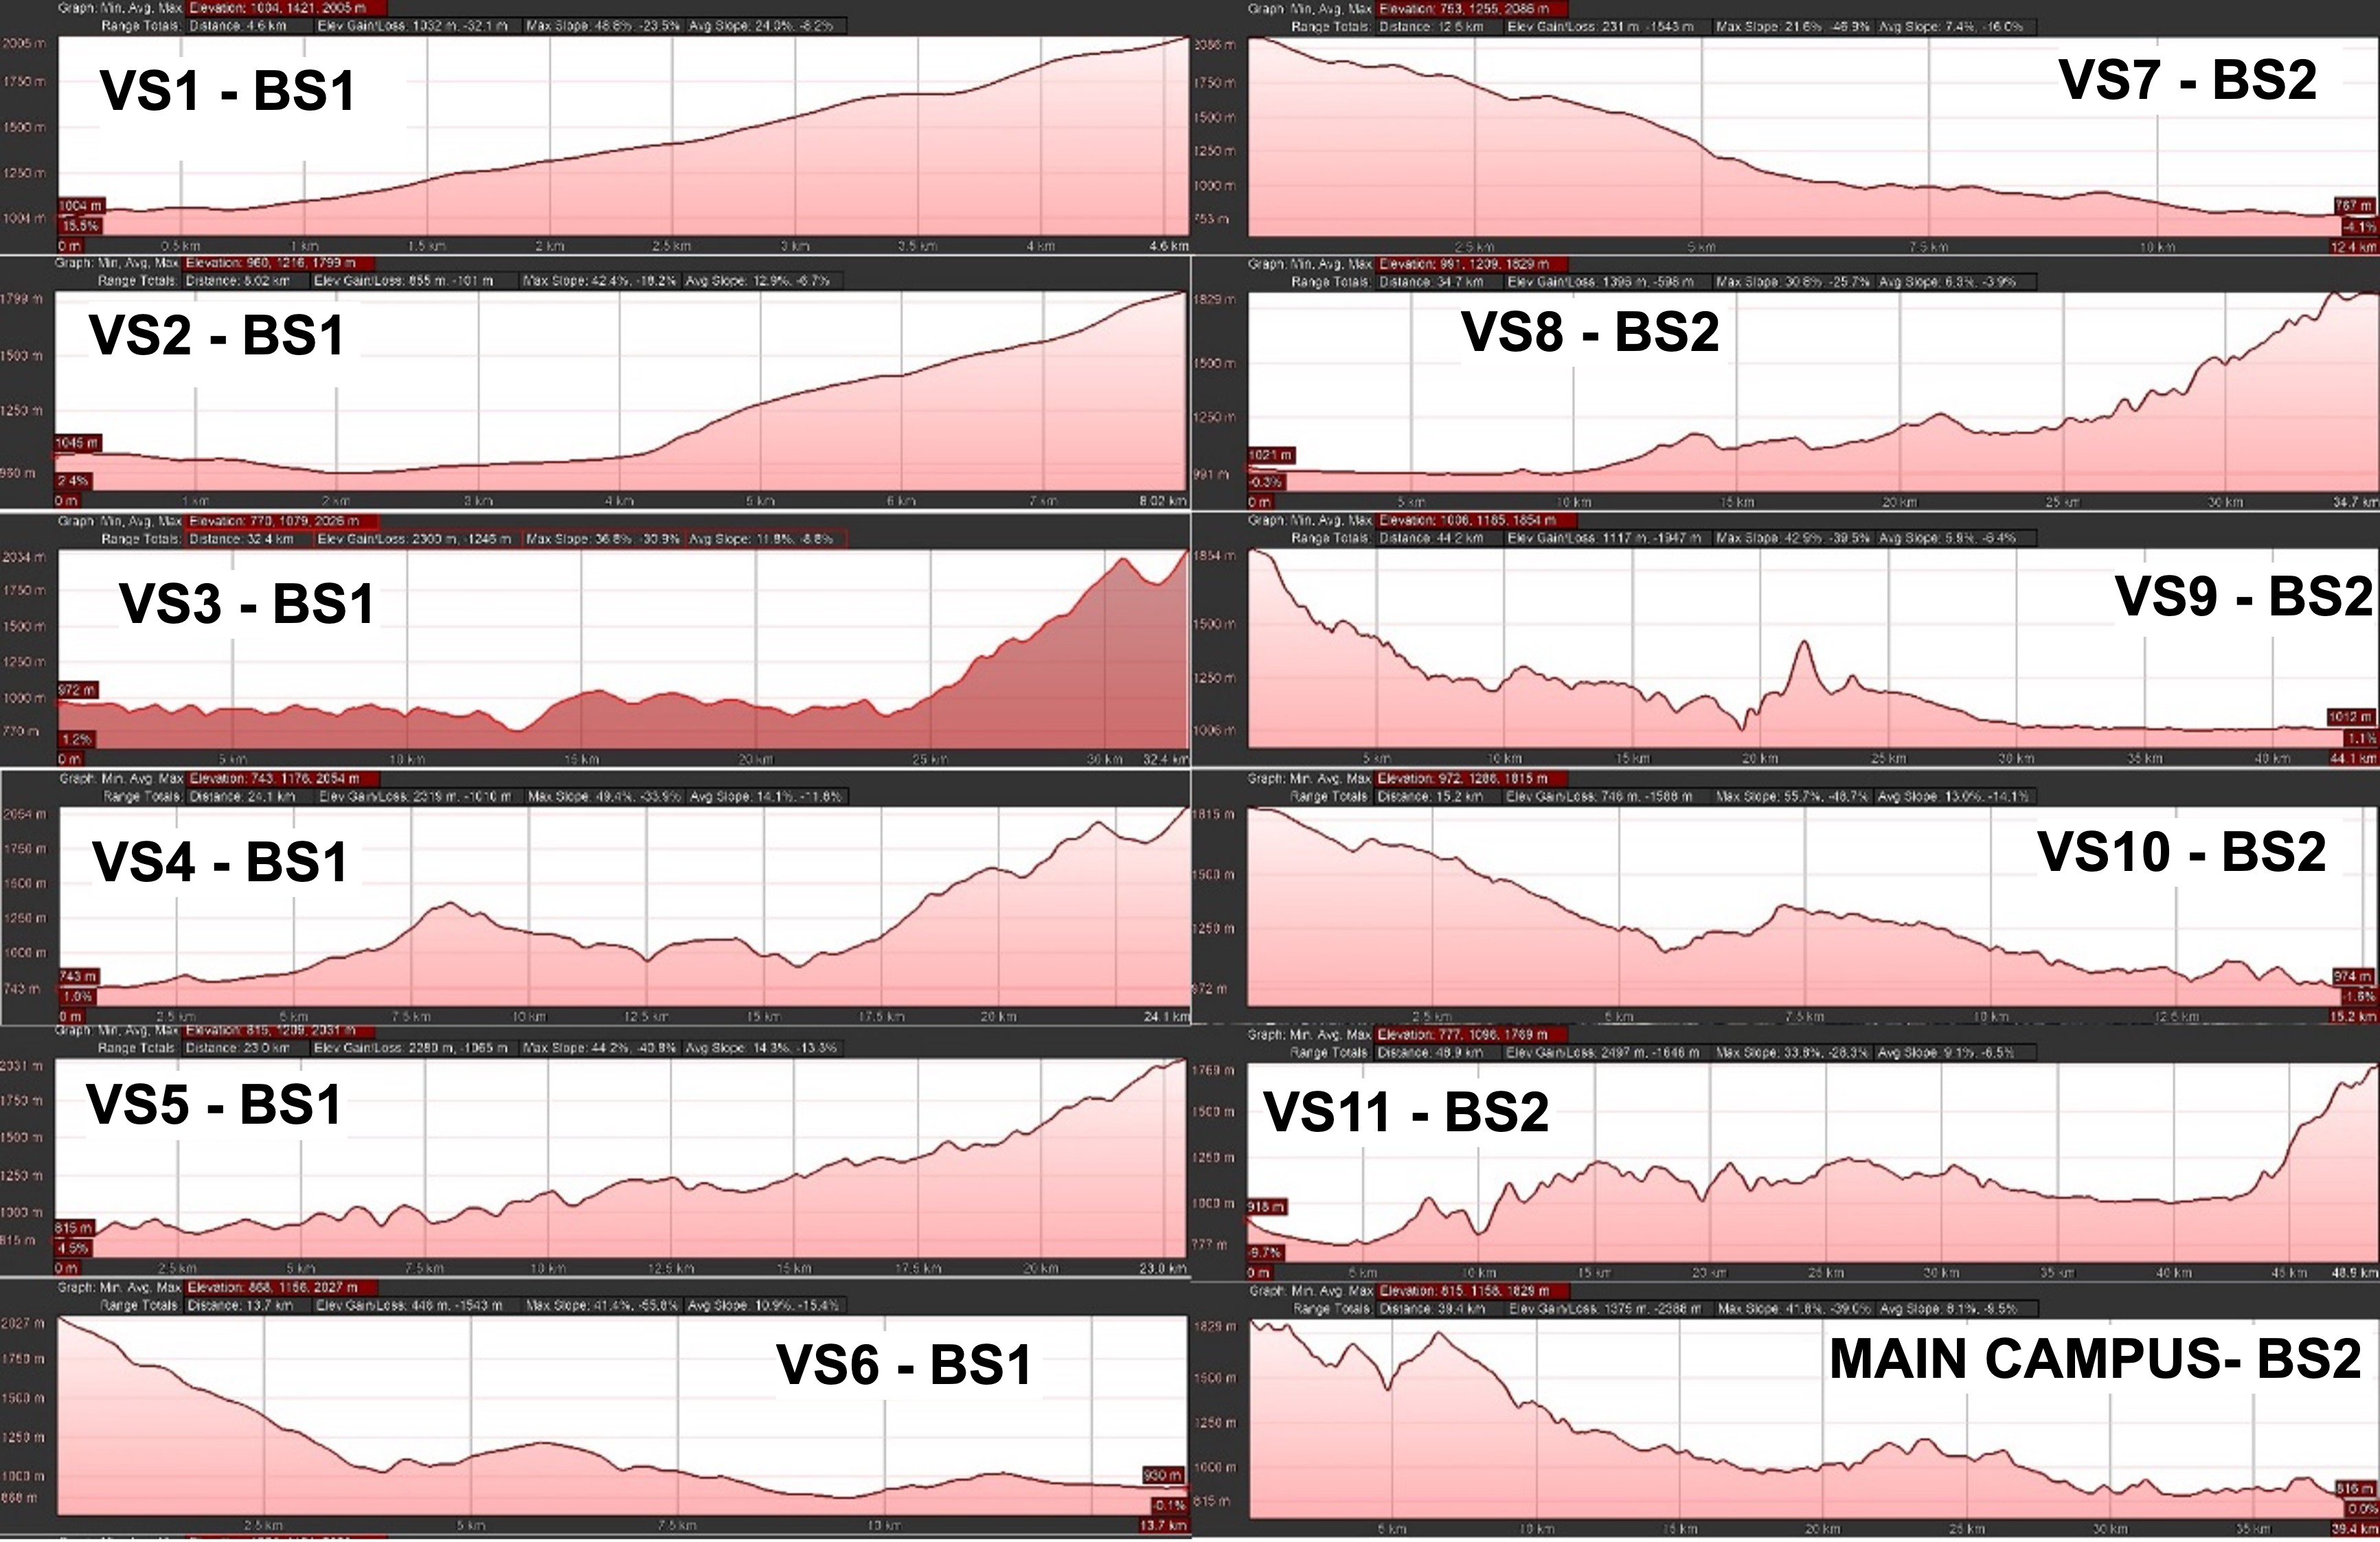
\includegraphics[width=\columnwidth]{figure2_REV.jpg}}
\caption{Altitude graphics between vocational schools and their connected base stations.}
\label{fig:figure2}
\end{figure}
\end{comment}
\section{Communication Network With Data Modelling}
The international standard IEC 61724 provides uniform information exchange for monitoring and controlling Photovoltaic farms. The focus of the IEC 61724 series is on communication between Photovoltaic plant components such as Photovoltaic panels and actors such as SCADA systems. Internal communication within Photovoltaic panel components is outside the scope of IEC61724 \cite{b7}\cite{b8}. Table \ref{tab:table1} shows the division of a Photovoltaic farm into logical nodes \cite{b7}. The logical node is a data holder that can hold different types of information related to the respective component.


\begin{table}[htbp]
\caption{Measuring Requirements for Sensor Data{\cite{b7}}}
\label{tab:table1}
\centering
\begin{tabular}{lllll}
\hline
Logic Node     & Unit & Sample Freq. & \#of Ch. & Data (B/s) \\ \hline
Temperature       & C    & 1 Hz         & 1            & 2             \\
Humidity          & \%   & 1 Hz         & 1            & 2             \\
Wind Speed        & m/s  & 3 Hz         & 1            & 6             \\
Global Irradiance & Wm\textsuperscript{-2}   & 100 Hz       & 1            & 200           \\
Voltage           & V    & 360 Hz       & 1            & 720           \\
Current           & A    & 360 Hz       & 1            & 720           \\ \hline
\end{tabular}
\end{table}


Riverbed modeler constructs the models by using an object-oriented modeling approach. Users can analyze simulated networks to compare the impact of different technology designs on end-to-end behavior. Moreover, the modeler incorporates a broad suite of protocols and technologies and includes a development environment to model all network types and technologies \cite{b9}.


According to IEC 61724 standard, Photovoltaic can be viewed as a logical device decomposed into logical nodes such as temperature, voltage, current, wind speed, and global irradiance. Fig.~\ref{fig:figure3} shows the proposed Riverbed logical node of a Photovoltaic system. Small scale Photovoltaic system consists of 24 logical nodes listed in Table2. All logical nodes send data to a local access point then the data are routed to a CCCL on the main campus of Kütahya Dumlupinar University by WiMAX communication system.

\begin{figure}[htbp]
\centerline{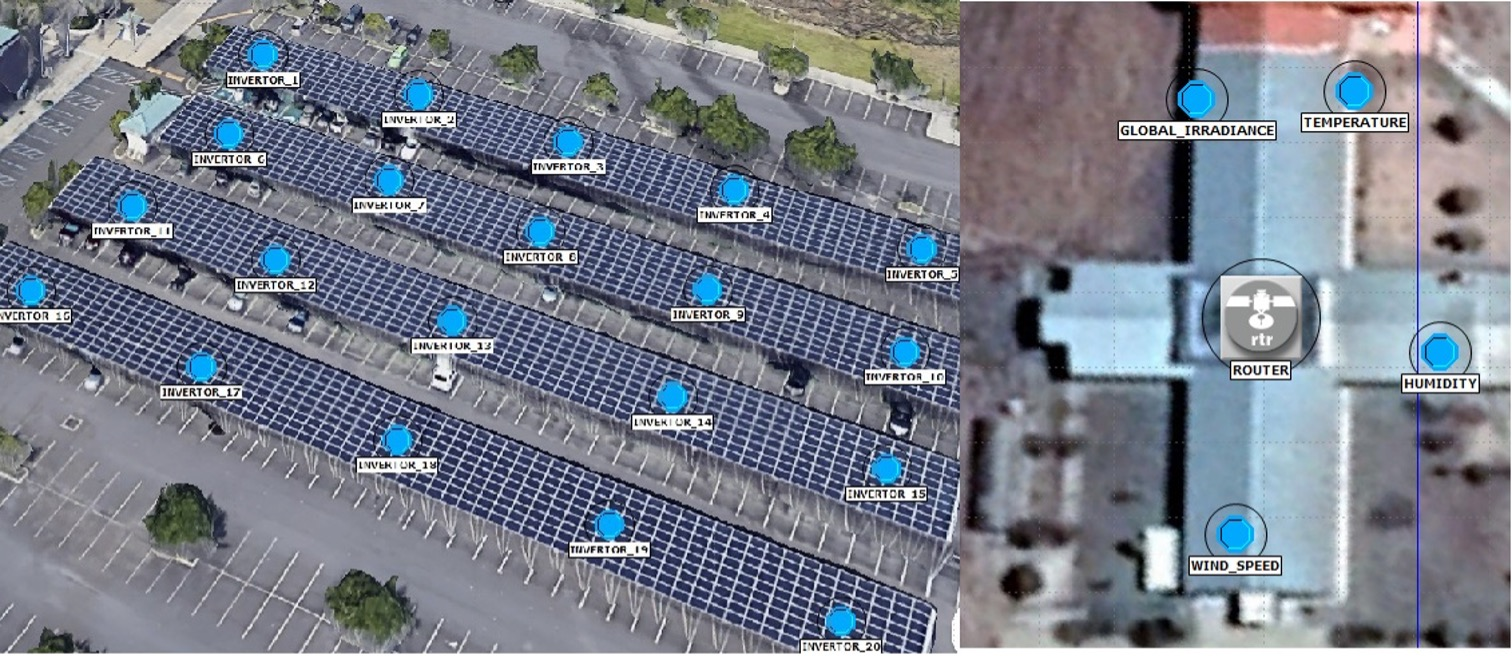
\includegraphics[width=\columnwidth]{figure3.jpg}}
\centering
\caption{WiFi network architecture of a vocational school in Riverbed Modeler.}
\label{fig:figure3}
\end{figure}

\subsection{Data Size Calculation}\label{AA}

This part describes the different quantities to be measured to perform condition monitoring and fault prediction tasks for a Photovoltaic system. Electrical quantities are voltage and current, and meteorology quantities are global irradiance, wind speed, humidity, and temperature. More detailed measurements and sensor technologies for a condition monitoring system in photovoltaic power plants are described in \cite{b8}.

Suppose a monitoring instrument inside the Photovoltaic inverter module samples different measurements, and each sample of data is represented by 2 Bytes. The data rate (Byte/s) can be calculated according to Eq. \eqref{eq1} \cite{b7}.

\begin{equation}
\text{Data Rate (Byte/s)} = 2.N\textsubscript{c}.f\textsubscript{s}\label{eq1}
\end{equation}

Where N\textsubscript{c} is the number of channels for a measuring quantity, and f\textsubscript{s} is the sampling frequency. For example, in the case of current data in an inverter, the monitoring instrument generates 360 samples/s with one channel, then the total amount of data is 360 samples/s. Each sample is represented by 2 Bytes then; the total is 720 B/s. Another example, in the case of global irradiance, the monitoring instrument generates 100 samples/s with one channel. Thus, the total sampling rate is 100 samples/s. Each sample is represented by 2 Bytes, then the total amount of data is 400 B/s, which matches the assumption given by reference \cite{b8}.

\begin{table}[htbp]
\caption{Data rate table from one vocational school}
\label{tab:table3}
\centering
\begin{tabular}{lccc}
\hline
\multicolumn{1}{c}{Logical Node} & \multicolumn{1}{l}{Data (Byte/s)} & \multicolumn{1}{l}{Quantitiy} & \multicolumn{1}{l}{Total Data (Byte/s)} \\ \hline
Temperature                      & 2                                 & 1                             & 2                                       \\
Humidity                         & 2                                 & 1                             & 2                                       \\
Wind Speed                       & 6                                 & 1                             & 6                                       \\
Global Irradiance                & 200                               & 1                             & 200                                     \\
Inverter                          & 1440                               & 20                            & 28800                                \\ \hline        
& & Total & 29010 \\
\end{tabular}
\end{table}


\subsection{Network Modeling}

There are eleven LPSL in this scenario. All LPSLs are identical except their locations. The solar panel area of each LPSL is 3 acres, and the generated power is 325 kW. LAN communication is configured to evaluate WiFi links. The main campus LAN (CCCL) contains a server and control center, for collecting and monitoring all Photovoltaic farm data. The vocational school Photovoltaic farms are sending their data over WiMAX network (RBSL). The topology is shown in Fig.~\ref{fig:figure1}.

\begin{table}[htbp]
\caption{The number of sensor nodes of all vocational schools and descriptions}
\centering
\label{tab:table8}
\begin{tabular}{ccc}
\hline
\begin{tabular}[c]{@{}c@{}}Sensor\\ Node\end{tabular} &
  \begin{tabular}[c]{@{}c@{}}Total\\ Number\end{tabular} &
  Comments \\ \hline
\begin{tabular}[c]{@{}c@{}}Inverter\\ Module\end{tabular} &
  220 &
  \begin{tabular}[c]{@{}c@{}}It has Voltage \& Current\\ sensor nodes\end{tabular} \\
\begin{tabular}[c]{@{}c@{}}Wind\\ Speed\end{tabular} &
  11 &
  \begin{tabular}[c]{@{}c@{}}Wind speed data\\ of vocational school\end{tabular} \\
Irradiance  & 11 & Irradiance data of vocational school  \\
Temperature & 11 & Temperature data of vocational school \\
Humidity    & 11 & Humidity data of vocation school      \\ \hline
\end{tabular}
\end{table}

Table \ref{tab:table3} shows the production data rate in one vocational school. From Table \ref{tab:table3}, the total production data rate from all vocational schools is 319,110 Byte per second.

\begin{table}[htbp]

\caption{WiFi communication parameters in vocational school LAN network}
\centering
\label{tab:table2}
\begin{tabular}{lll}
\hline
\multicolumn{3}{c}{WiFi 802.11g}                             \\ \hline
                           & AP (Access Point) & Sensor Node \\
Tx Power                   & 1 W               & 1 W         \\
Data Rate                  & 50 Mbps           & 1 Mbps      \\
Receiver Power Threshold   & -95 dBm           & -95 dBm     \\
Buffer Size                & 1024000 bits      & 256000 bits \\
Short Retry Limit          & 7                 & 7           \\
Long Retry Limit           & 4                 & 9           \\
Large Packet Processing    & Fragment          & Fragment    \\
Access Point Functionality & Enabled           & Disabled   
\end{tabular}
\end{table}

%----------------------------------------------

\begin{table}[htbp]
\caption{Node Model Used in Riverbed Modeler Simulation}
\label{tab:table6}
\centering
\begin{tabular}{lll}
\hline
\multicolumn{1}{c}{Component Name} & \multicolumn{1}{c}{LPSL \& CCCL} & \multicolumn{1}{c}{RBSL}                                                      \\ \hline
Sensor Node & wlan\_wkstn\_adv   & -- \\
Data Collection Unit               & wlan\_slip4\_adv                 & \begin{tabular}[c]{@{}l@{}}ss\_wimax\_router\\ wimax\_bs\_router\end{tabular} \\
Main Server & wlan\_server model & -- \\ \hline
\end{tabular}
\end{table}
%----------------------------------------------




Tables \ref{tab:table2} and \ref{tab:table4} show WiFi and WiMAX configurations on Riverbed Modeler software. Fig.~\ref{fig:figure3} shows the communication network model of vocational schools and the main campus on Riverbed Modeler software. The university consists of 11 small-scaled Photovoltaic farms divided into 11 vocational school clusters. Fig.~\ref{fig:figure3} shows that each vocational school subnet consists of 24 logical nodes with a star topology. The main topology from Fig.~\ref{fig:figure1} shows the produced data from sensor nodes are being transmitted to the main server in CCCL. To implement the simulation, we used FTP type traffic model in Riverbed Modeler. The make a relaible communication, the upload response time plays significant role of our communication network architecture.
\begin{table}[htbp]
\caption{WİMAX configuration table}
\centering
\label{tab:table4}
\begin{tabular}{lc}
\hline
\multicolumn{1}{c}{Parameter} & Base Stations                 \\ \hline
Cell Radius                   & 40 km                         \\
HY Layer Profile              & OFDMA                         \\
Carrier Frequency             & 3.5 GHz                       \\
Channel Bandwidth             & 5.5 MHz                       \\
Number of Subscribers         & 7                             \\
Modulation and Coding         & 64 QAM                        \\
Duplexing Scheme              & TDD                           \\
BS/SS: Antenna Gain           & 20 dBi                        \\
BS/SS Transmission Power      & 10 W                          \\
Multipath Channel Model       & ITU Vehicular                 \\
Pathloss Channel Model        & Suburban Fixed (Erceg) Type-A \\ \hline
\end{tabular}
\end{table}

Time elapsed between sending a file and receiving the response packet for the FTP application defines the upload response time. FTP send data over TCP/IP connection. Table \ref{tab:table3} shows the data rate of sensor node data size for the status report related the photovoltaic farm production performance. The data were encapsulated to communicate in FTP standards. Table \ref{tab:table6} shows the node models which are used in Riverbed Modeler software to implement the FTP traffic 2 hopped hybrid communicationn scenario. 





\subsection{Communication Timing Requirements}
The IEC does not offer exact specific timing requirements for the solar power domain in this context of the photovoltaic power system communications network. To observe real time monitoring and controlling, we selected IEEE 1646 standard \cite{b10}. In our network model, the internal and external timing requirements for the power substation automation are considered to evaluate the network model, as shown in Table \ref{tab:table5}. 


\begin{table}[htbp]
\caption{IEEE 1646 communication timing requirements for electric substation automation}
\centering
\label{tab:table5}
\begin{tabular}{lcl}
\hline
\multicolumn{1}{c}{Application} & Internal & External  \\ \hline
Protection                      & 4 ms     & 8 - 12 ms \\
Monitoring and Control          & 16 ms    & 1 s       \\
Operation and Maintenance       & 1 s      & 10 s      \\
Audio and Video                 & 1 s      & 1 s      \\ \hline
\end{tabular}
\end{table}

\section{Simulation Results and Analysis}


The performance of the proposed architecture was evaluated by simulating different scenarios that considered small-scaled solar farms with eleven LPSLs, two RBSLs and one CCCL. Simulation results were verified by comparing the calculated data with the received data for a different types of information at servers. The sent traffic at LPSL local server is shown in Table \ref{tab:ResultTable} which the total data rate is 29,010 B/s is identical to Table \ref{tab:table3}.



\begin{comment}

\begin{figure}[htbp]
%LPSL server income data plotting section
\pgfplotsset{every axis/.append style={
font=\footnotesize,
thin,
tick style={ultra thin}},
}
    \begin{tikzpicture}
\begin{semilogyaxis}[ymax = 20000.0000000,
xlabel={Simulation Duration (Seconds)},
ylabel={Received Data Size (Byte)},
xmode=normal, ymode=log, 
grid = major,
log ticks with fixed point,
ytick={2,6,200,14400},
transpose legend,
legend columns = 2,
legend style = {font=\tiny,at={(1,0.8)}, anchor=east}
]


\addplot [color=blue, mark=oplus*, mark repeat =14, mark size = 3]  table [x = Simulation Duration, y = Received Current Data, col sep = comma] {fig4deneme (1).csv};





%--
\addplot [color=yellow, mark=pentagon*, mark repeat =14, mark size = 3, mark phase = 8]  table [y = Received Voltage Data, col sep = comma] {fig4deneme (1).csv};

%--
\addplot [color = red, dotted, mark=otimes*, mark repeat =14, mark size = 3,mark phase = 8 ] table [y = Received Temperature Data, col sep = comma] {fig4deneme (1).csv};

%--
\addplot [color = green, dotted, mark=diamond*, mark repeat =14, mark size = 3, ]table [y = Received Humidty Data, col sep = comma] {fig4deneme (1).csv};

%--
\addplot [color=orange, mark=square*, mark repeat =14, mark size = 3]table [y = Received Wind Speed Data, col sep = comma] {fig4deneme (1).csv};

%---
\addplot [color=violet, mark=triangle*, mark repeat =14, mark size = 3] table [y = Received Global Irradiance Data, col sep = comma] {fig4deneme (1).csv};

\legend{Current Data,Voltage Data,Temperature Data,Humidity Data,Wind Speed Data,Irradiance Data}

\end{semilogyaxis}
\end{tikzpicture}

\caption{Received data rate of LPSL server in simulation duration. }
\label{fig:figure4}
\end{figure}
\end{comment}



\begin{table}[htbp]
\centering
\caption{Simulation results on Riverbed Modeler.}
\label{tab:ResultTable}
\begin{tabular}{ccc}
\hline
Component & \begin{tabular}[c]{@{}c@{}}LPSL\\ Server\end{tabular} & \begin{tabular}[c]{@{}c@{}}CCCL\\ Server\end{tabular} \\ \hline
Humidity          & 2 B/s      & 22 B/s      \\
Temperature       & 2 B/s      & 22 B/s      \\
Wind Speed        & 6 B/s      & 66 B/s      \\
Voltage           & 14.400 B/s & 158.000 B/s \\
Current           & 14.400 B/s & 158.000 B/s \\
Global Irradiance & 200 B/s    & 2.200 B/s   \\ \hline
TOTAL & 29.010 B/s    & 318.310 B/s   \\ \hline
\end{tabular}
\end{table}


\begin{comment}

\begin{figure}[htbp]
%CCCL server income data plotting section
\pgfplotsset{every axis/.append style={
font=\footnotesize,
thin,
tick style={ultra thin}},
}
    \begin{tikzpicture}
\begin{semilogyaxis}[ymax = 200000.0000000,
xlabel={Simulation Duration (Seconds)},
ylabel={Received Data Size (Byte)},
xmode=normal, ymode=log, 
grid = major,
log ticks with fixed point,
ytick={22,66,2200,158400},
transpose legend,
legend columns = 2,
legend style = {font=\tiny,at={(1,0.8)}, anchor=east}
]


\addplot [color=blue, mark=oplus*, mark repeat =14, mark size = 3]  table [x = Simulation Duration, y = ToCurrent, col sep = comma] {fig4deneme (1).csv};


%--
\addplot [color=yellow, mark=pentagon*, mark repeat =14, mark size = 3, mark phase = 8]  table [y = ToVoltage, col sep = comma] {fig4deneme (1).csv};

%--
\addplot [color = red, dotted, mark=otimes*, mark repeat =14, mark size = 3,mark phase = 8 ] table [y = ToTemp, col sep = comma] {fig4deneme (1).csv};

%--
\addplot [color = green, dotted, mark=diamond*, mark repeat =14, mark size = 3, ]table [y = ToHum, col sep = comma] {fig4deneme (1).csv};

%--
\addplot [color=orange, mark=square*, mark repeat =14, mark size = 3]table [y = ToWind, col sep = comma] {fig4deneme (1).csv};

%---
\addplot [color=violet, mark=triangle*, mark repeat =14, mark size = 3] table [y = ToRad, col sep = comma] {fig4deneme (1).csv};


\legend{Current Data,Voltage Data,Temperature Data,Humidity Data,Wind Speed Data,Irradiance Data}


\end{semilogyaxis}
\end{tikzpicture}

\caption{The collection of all vocational schools' sensor data to CCCL server}
\label{fig:figure6}
\end{figure} 
\end{comment}

\begin{comment}

\begin{figure}[htbp]
%Upload ResponseTime Section 
\pgfplotsset{every axis/.append style={
font=\footnotesize,
thin,
tick style={ultra thin}},
}
    \begin{tikzpicture}
\begin{axis}[
xlabel={Simulation Duration (Seconds)},
ylabel={Upload Response Time},
grid,
legend style = {font=\tiny,at={(1,0.9)}, anchor=east}
]

\addplot [color=cyan, mark=star, mark repeat =14, mark size = 3] table [x = Simulation Duration, y = Up Time, col sep = comma] {fig4deneme (1).csv};
\legend{Upload Response Time}



\end{axis}
\end{tikzpicture}

\caption{Average upload response time of vocational school's sensor nodes to LPSL server}
\label{fig:figure5}
\end{figure}
\end{comment}


The received traffic at CCCL central server is shown in Table \ref{tab:ResultTable} which the total data rate is 319.310 B/s. The WAN scenario results are identical to the calculation mentioned in the previous section. 

The delay time in WiMAX communication represents the end-to-end delay of all the packets received by the WiMAX MACs of all WiMAX nodes in the network and forwarded to the higher layer. The delay time in WiFi communication represents the end to end delay of all the packets received by the wireless LAN MACs of all WLAN nodes in the network and forwarded to the higher layer. This delay includes medium access delay at the source MAC, reception of all the fragments individually, and transfer of the frames via access point, if access point functionality is enabled.
The global delay results in WiFi and WiMAX results are shown in Table \ref{tab:table7}. 



\begin{comment}

\begin{figure}[htbp]
%End To End  Section 
\pgfplotsset{every axis/.append style={
font=\footnotesize,
thin,
tick style={ultra thin}},
scaled y ticks=false,
yticklabel style = {
/pgf/number format/fixed,
/pgf/number format/precision=5
},
}
    \begin{tikzpicture}
\begin{semilogyaxis}[
xlabel={Simulation Duration (Seconds)},
ylabel={End To End Delay Time (Seconds)},
xmode=normal, ymode=log, 
grid = major,
log ticks with fixed point,
legend style = {font=\tiny,at={(1,0.8)}, anchor=east}
]

\addplot [color=orange, mark=pentagon*, mark repeat =14, mark size = 3]  table [x = Simulation Duration, y = wimax, col sep = comma] {fig4deneme (1).csv};
\addlegendentry{WiMAX}
\addplot [color=blue, mark=star, mark repeat =14, mark size = 3]  table [x = Simulation Duration, y = wlan, col sep = comma] {fig4deneme (1).csv};
\addlegendentry{WiFi}


\end{semilogyaxis}
\end{tikzpicture}

\caption{Average End to End delay results of the WAN and LAN network layers}
\label{fig:figure7}
\end{figure}
\end{comment}

\begin{table}[htbp]
\caption{End to end delay performance of the simulation}
\centering
\label{tab:table7}
\begin{tabular}{ccccc}
\hline
\begin{tabular}[c]{@{}c@{}}Simulation\\Results\end{tabular} &
  \begin{tabular}[c]{@{}c@{}}Mean\\Delay(s)\end{tabular} &
  \begin{tabular}[c]{@{}c@{}}Variance\\ (s)\end{tabular} &
  \begin{tabular}[c]{@{}c@{}}Std\\Deviation (s)\end{tabular} &
  \begin{tabular}[c]{@{}c@{}}Correlation\\Coefficient\end{tabular} \\ \hline
WiFi &
  0.001532 &
  3.30x10\textsuperscript{-11} &
  5.74x10\textsuperscript{-6} &
  \multirow{2}{*}{-0.58613} \\
WiMAX &
  0.044164 &
  1.16x10\textsuperscript{-10} &
  1.08x10\textsuperscript{-5} &
   \\ \hline
\end{tabular}
\end{table}

The vocational schools' average upload response time results is shown in Fig.~\ref{fig:figure10}. It's an expected result, because the vocational school data need to travel two more layer to reach the CCCL server.  

\begin{figure}[htbp]
%TotalUploadResponse
\pgfplotsset{every axis/.append style={
font=\footnotesize,
thin,
tick style={ultra thin}},
scaled y ticks=false,
yticklabel style = {
/pgf/number format/fixed,
/pgf/number format/precision=5
},
}

    \begin{tikzpicture}
    \begin{axis}[
    xlabel={Simulation Duration (Seconds)},
    ylabel={Upload Response Time (Seconds)},
    grid,
    legend style = {font=\tiny,at={(1,0.8)}, anchor=east}
    ]

\addplot [color=cyan, mark=star, mark repeat =14, mark size = 3]  table [x = Simulation Duration, y = totalUpload, col sep = comma] {fig4deneme (1).csv};
\addlegendentry{Upload Response Time}



\end{axis}
\end{tikzpicture}
\caption{Upload response time (seconds) from all vocational schools' sensor nodes to CCCL server}
\label{fig:figure10}
\end{figure}




\section*{Conclusion § Future Work}

We have proposed a hierarchical communications network architecture for small-scale Photovoltaic farms in this work. The Riverbed modeler was used to model and simulate the network, and the communications network models were validated by measuring the amount of traffic received at the CCCL. We investigated the network delay and upload response time of eleven vocational school Photovoltaic systems. The simulation results satisfy the timing requirements of IEEE 1646 standards for automation monitoring systems and also satisfy the IEC 61724 standards for monitoring and control the Photovoltaic systems for the application. Our future work will extend the network model for hybrid large-scale Photovoltaic and wind turbine systems by using a wireless-based distributed sensor system solution.  

\begin{thebibliography}{00}
%\bibitem{b1} “Wisconsin K-12 Energy Education Program,” UWSP. [Online]. Available: https://www3.uwsp.edu/cnr-ap/keep/Pages/default.aspx. [Accessed: 30-May-2022]. 
\bibitem{b2} A. Garro and F. Barrara, “Reliability analysis of residential photovoltaic systems,” Renewable Energy and Power Quality Journal, pp. 1197–1202, 2011. 
\bibitem{b3} S. S. Hussain, K. S. Khattak, A. Khan, and Z. H. Khan, “Cyber physical system for solar energy monitoring,” 2019 International Conference on Frontiers of Information Technology (FIT), 2019. 
\bibitem{b4} B. K. Singh, J. Coulter, M. A. Sayani, S. M. Sami, M. Khalid, and K. E. Tepe, “Survey on communication architectures for wind energy integration with the smart grid,” International Journal of Environmental Studies, vol. 70, no. 5, pp. 765–776, 2013.
\bibitem{b5} A. J. Abid, R. S. Ali, F. M. Al-Naima, Z. Ghassemlooy, and Z. Gao, “A new power line communication modem design with applications to vast solar farm management,” 2013 3rd International Conference on Electric Power and Energy Conversion Systems, 2013.
\bibitem{b6} M. A. Ahmed and K. Young-Chon, “Communication networks of domestic small-scale renewable energy systems,” 2013 4th International Conference on Intelligent Systems, Modelling and Simulation, 2013.
\bibitem{b7} M. Ahmed, Y. Kang, and Y.-C. Kim, “Communication network architectures for smart-house with Renewable Energy Resources,” Energies, vol. 8, no. 8, pp. 8716–8735, 2015.
\bibitem{b8} Standards Australia Limited., \& Standards New Zealand,. (2020). Photovoltaic system performance. 
\bibitem{b9} RIVERBED MODELER: Discrete Event Simulator for Network Simulation: Riverbed
\bibitem{b10} IEEE Std 1646-2004: IEEE Standard Communication Delivery Time Performance Requirements for Electric Power Substation Automation. (2005). Place of publication not identified: IEEE.
\bibitem{b11} M. Ahmed and Y.-C. Kim, “Communication network architectures for  smart-wind power farms,” Energies, vol. 7, no. 6, pp. 3900–3921, 2014.


\end{thebibliography}


\end{document}



